\chapter{Resultados}

%\noindent En este último capítulo se analiza los resultados del caso del Sorteo Tec en dos partes: la dimensión nacional y la internacional. 

\newpage

\section{El Sorteo Tec}

%Analisis de valor esperado de los diferentes sorteos

\noindent A continuación, pasaremos al análisis de aversión al riesgo de las diferentes loterías. Se cuenta con la información relacionada al número de premios, el valor de los premios y el número de boletos emitidos en cada sorteo, con esta información se obtuvieron las probabilidades asociadas a cada premio y así definir la lotería $L$ como se mencionó en el capítulo \textbf{2.1}. \\

Para el sorteo \textbf{AventuraT} se tiene una emisión de 60,000 boletos y hay un total de 6,421 premios. Con esta información sabemos que la probabilidad de ganar alguno de los premios es de 0.10702.

\begin{table}[H]
\centering
\caption{Información sorteo AventuraT}
\label{tab:avent}
\begin{tabular}{@{}lll@{}}
\toprule
\multicolumn{1}{c}{Premios} & \multicolumn{1}{c}{\$} & \multicolumn{1}{c}{Probabilidad} \\ \midrule
1                           & 1,000,000                & 0.00001666666667                 \\
1                           & 100,000                 & 0.00001666666667                 \\
1                           & 50,000                  & 0.00001666666667                 \\
3                           & 20,000                  & 0.00005                          \\
10                          & 5,000                   & 0.0001666666667                  \\
25                          & 2,500                   & 0.0004166666667                  \\
80                          & 1,000                   & 0.001333333333                   \\
300                         & 500                    & 0.005                            \\
6,000                        & 140                    & 0.1                              \\ \bottomrule
\end{tabular}
\end{table}

Además, se obtuvo el valor esperado de esta lotería. El resultado fue $E[L] =$ 39.88, menor al valor del boleto que es de $\$ 140$. \\ \\\\

Para el sorteo \textbf{Educativo} se tiene una emisión de 470,000 y un total de 26, 835 premios. Con esta información sabemos que la probabilidad de ganar alguno de los premios es de 0.05710

\begin{table}[H]
\centering
\caption{Información sorteo Educativo}
\label{tab:educ}
\begin{tabular}{@{}lll@{}}
\toprule
\multicolumn{1}{c}{Premios} & \multicolumn{1}{c}{\$} & \multicolumn{1}{c}{Probabilidad} \\ \midrule
1                           & 12,000,000               & 0.000002127659574                \\
2                           & 1,045,000                & 0.000004255319149                \\
7                           & 1,000,000                & 0.00001489361702                 \\
10                          & 100,000                 & 0.00002127659574                 \\
15                          & 50,000                  & 0.00003191489362                 \\
100                         & 5,000                   & 0.0002127659574                  \\
400                         & 2,500                   & 0.0008510638298                  \\
2,800                        & 1,000                   & 0.005957446809                   \\
23,500                       & 300                    & 0.05                             \\ \bottomrule
\end{tabular}
\end{table}

\newpage
Para el sorteo \textbf{Mi Sueño} se tiene una emisión de 280,000 boletos y hay un total de 19,950 premios. Con esta información sabemos que la probabilidad de ganar alguno de los premios es de 0.07125. 

\begin{table}[H]
\centering
\caption{Información sorteo Mi Sueño}
\label{tab:misuen}
\begin{tabular}{@{}lll@{}}
\toprule
\multicolumn{1}{c}{Premios} & \multicolumn{1}{c}{\$} & \multicolumn{1}{c}{Probabilidad} \\ \midrule
1                           & 28,000,000               & 0.000003571428571        \\
1                           & 5,333,280                & 0.000003571428571        \\
1                           & 1,800,000                & 0.000003571428571        \\
7                           & 100,000                 & 0.000025                 \\
10                          & 50,000                  & 0.00003571428571         \\
50                          & 10,000                  & 0.0001785714286          \\
280                         & 5,000                   & 0.001                    \\
2,800                        & 1,650                   & 0.01                     \\
5,600                        & 1,100                   & 0.02                     \\
11,200                       & 600                    & 0.04                     \\ \bottomrule
\end{tabular}
\end{table} \\

Además, con esta información podemos obtener el valor esperado de esta lotería. Así obtenemos que $E[L] = $ 199.05, menor al valor del boleto que es de $\$ 600$. 

\newpage
Para el sorteo \textbf{Tradicional} se tiene una emisión de 250,000 boletos y un total de 12,323 premios. Con esta información sabemos que la probabilidad de ganar alguno de los premios es de 0.04929.

\begin{table}[H]
\centering
\caption{Información sorteo Tradicional}
\label{tab:trad}
\begin{tabular}{@{}lll@{}}
\toprule
\multicolumn{1}{c}{Premios} & \multicolumn{1}{c}{\$} & \multicolumn{1}{c}{Probabilidad} \\ \midrule
1                           & 60,750,000               & 0.000004                         \\
1                           & 8,500,000                & 0.000004                         \\
1                           & 3,226,000                & 0.000004                         \\
1                           & 1,100,000                & 0.000004                         \\
1                           & 949,900                 & 0.000004                         \\
1                           & 841,000                 & 0.000004                         \\
1                           & 719,900                 & 0.000004                         \\
1                           & 495,000                 & 0.000004                         \\
80                          & 100,000                 & 0.00032                          \\
100                         & 20,000                  & 0.0004                           \\
400                         & 5,000                   & 0.0016                           \\
1,735                        & 2,500                   & 0.00694                          \\
10,000                       & 1,100                   & 0.04                             \\ \bottomrule
\end{tabular}
\end{table}

Además, como esta información podemos obtener el valor esperado de esta lotería. Así obtenemos que $E[L] = $ 415.68, menor al valor del boleto que es de $\$ 1100$. \\

%Esto no estoy muy seguro de dejarlo
\newpage

Ahora bien, el valor esperado de cada lotería y las probabilidades que hay de ganar un premio nos hacen remarcar lo siguiente: las apuestas con probabilidad de ganar ($p$) pequeñas resultan menos atractivas de lo que deberían para un individuo que maximiza su utilidad. De aquí que la forma en que se utilizan los pesos para calcular tanto el valor esperado como la utilidad esperada generan una fuente de aversión al riesgo (O’Donoghue y Somerville, 2018). \\

Por otro lado, la aversión al riesgo deriva de la utilidad marginal decreciente que existe por la riqueza monetaria. Supongamos a dos individuos con diferentes riquezas tales que la riqueza de uno es mayor que del otro. Sea $W_a$ y $W_b$ las riquezas para los individuos A y B respectivamente y que $W_a < W_b$, además bajo el supuesto que estos dos individuos son aversos al riesgo la utilidad que le daría ganar un premio al individuo A es mayor a la utilidad que le daría ganar un premio al individuo B. \\

\newpage

Esto se debe a la concavidad de la función de utilidad que representa a los individuos aversos al riesgo, la pendiente en el punto $M$ es mayor a la pendiente en el punto $N$ y esto nos explica la forma en que la utilidad aumenta en cada caso. Gráficamente se ve de la siguiente manera:

\begin{figure}[H]
    \centering
    \caption{Comparación dos individuos}
    \label{fig:my_label}
    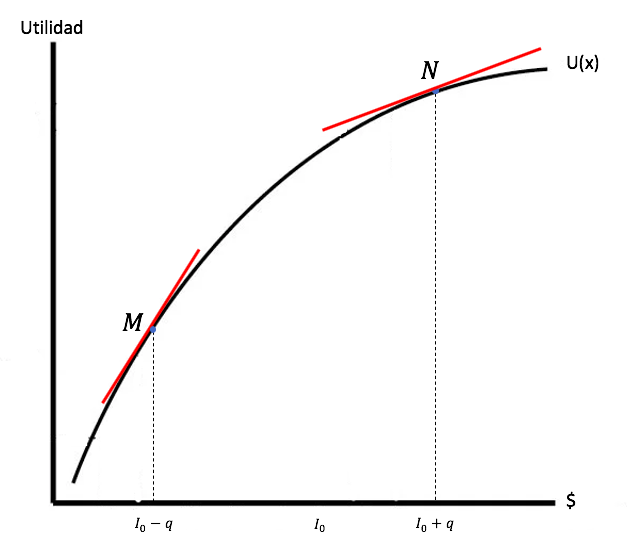
\includegraphics[width=.85\linewidth]{Imagenes/UE_MN.png} \\
    \imagesource{Elaboración propia}
\end{figure}




\newpage
%%Analisis de resultados del modelo econometrico

Pasemos ahora a analizar los resultados obtenidos de nuestros modelos. Como mencionamos en el capítulo anterior, los coeficientes relevantes resultan ser $\beta_1$ para el modelo (3.1) y $\beta_2$ para el modelo (3.2). Retomemos los resultados obtenidos de estos modelos:

\begin{table}[H]
\centering
\caption{Resumen coeficientes}
\label{tab:my-table}
\begin{tabular}{lcccc}
\hline
      & \multicolumn{1}{l}{AventuraT} & \multicolumn{1}{l}{Educativo} & \multicolumn{1}{l}{Mi sueño} & \multicolumn{1}{l}{Tradicional} \\ \hline
\multicolumn{5}{c}{Modelo (3.1)}                                                                                                       \\
\beta_1 & 1.542                         & 1.726                         & 1.854                        & 1.751                           \\ \hline
\multicolumn{5}{c}{Modelo (3.2)}                                                                                                       \\
\beta_2 & $-$1.613e-07 & $-$5.713e-07  & $-$2.588e-07   & $-$2.253e-07 \\              
\end{tabular}
\end{table}

Observamos que, para todos los sorteos el coeficiente $\beta_1 > 1$ lo que nos indica que las elasticidad ingreso de los boletos del Sorteo Tec es mayor a uno. Por otro lado, todos los coeficientes fueron estadísticamente diferentes de 0 a excepción de $\beta_2$ para el sorteo Tradicional. \\

\begin{equation*}
     \beta_1 > 1
\end{equation*}
\begin{equation*}
    \Rightarrow \varepsilon_{I,x} > 1
\end{equation*}
\begin{equation*}
    \Rightarrow \frac{\Delta\% Boletos}{\Delta \% PIB pc} >1
\end{equation*} 

\newpage

Esto nos indica que el bien es un \textbf{bien superior al ingreso}, lo cual se traduce que ante un cambio en el PIB \textit{per capita} el cambio en el número de boletos será mayor en valor absoluto. Este resultado va en línea con nuestra hipótesis, sustentando nuestra idea inicial que ante disminuciones en el ingreso la cantidad demanda de boletos disminuye. Esto aplica para los cuatro sorteos sobre los cuales se realizó el análisis.  \\

\begin{table}[H]
\centering
\begin{tabular}{l|ll}
\cline{1-1}
\downarrow I \Rightarrow \ \downarrow X  &   &   \\
          & = & \mid \Delta X| > |\Delta I| \\
\uparrow I \Rightarrow \ \uparrow X &   &   \\ \cline{1-1}
\end{tabular}
\end{table} 

\begin{figure}[H]
\centering
\caption{Relación \beta_1}
\label{fig:test}
\begin{subfigure}
  \centering
  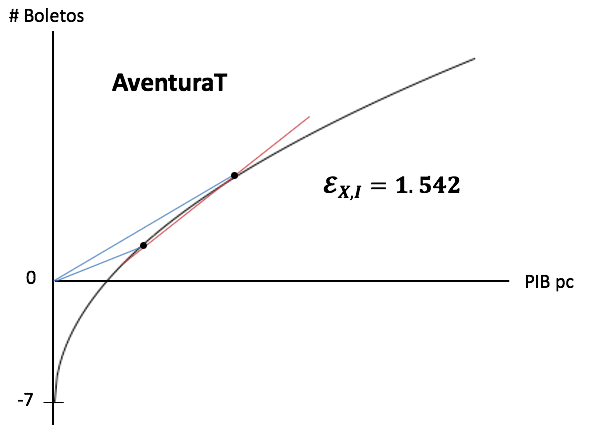
\includegraphics[width=.45\linewidth]{Imagenes/aven.png}
\end{subfigure}%
\begin{subfigure}
  \centering
  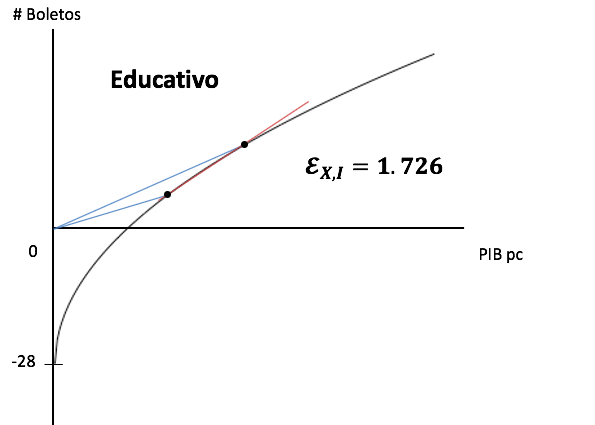
\includegraphics[width=.45\linewidth]{Imagenes/educ.png}
\end{subfigure}
\end{figure}

\begin{figure}[H]
\centering
\begin{subfigure}
  \centering
  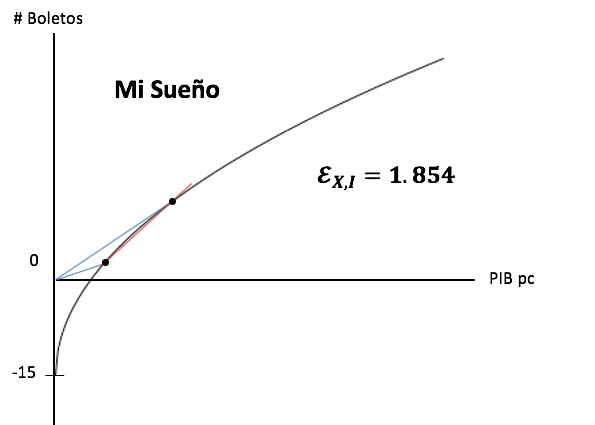
\includegraphics[width=.45\linewidth]{Imagenes/suen.png}
\end{subfigure}%
\begin{subfigure}
  \centering
  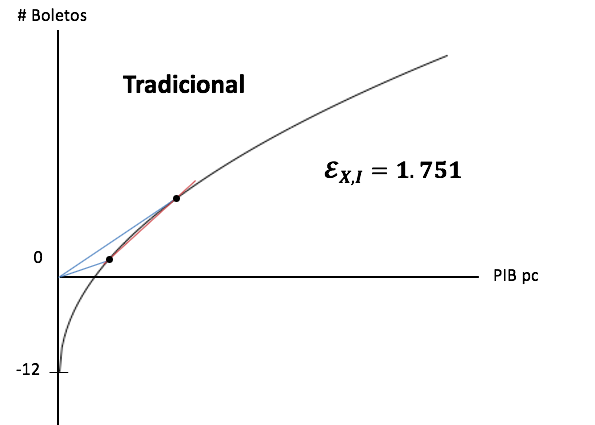
\includegraphics[width=.45\linewidth]{Imagenes/trad.png}
\end{subfigure}
\end{figure}

\newpage

Por otro lado, el coeficiente $\beta_2$ nos dice si la función es cóncava o convexa. Como se mencionó anteriormente, un individuo que es averso al riesgo tiene preferencias cóncavas ($U^{\prime \prime} < 0$). Para todos los sorteos el coeficiente $\beta_2$ es negativo pero muy cercano a cero, lo cual nos dice que los individuos son aversos al riesgo aunque la relación es casi lineal, consistente con el hecho que los bienes son superiores al ingreso. Además, al aumentar el ingreso la curva de utilidad se aplana lo cual implica que la curva es cóncava. Lo anterior nos vuelve a confirmar que los individuos que participan en estas loterías son aversos al riesgo. \\

\begin{figure}[H]
    \centering
    \caption{Relación \beta_2}
    \label{fig:my_label}
    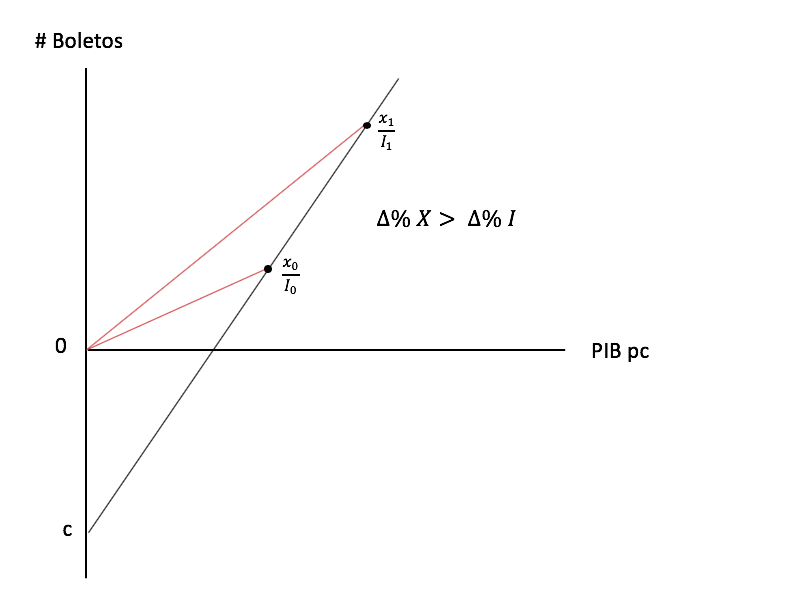
\includegraphics[width=.85\linewidth]{Imagenes/sorteo_gen2.png}
\end{figure} \\

\newpage

%Checar si esto lo puedo poner en otra parte


Se obtuvo información\footnote{Información publicada el 22 de abril de 2020 en la platorma EIKON} sobre las estimaciones del PIB para 2020 de 35 diferentes instituciones, dichas instituciones publican la variación anual que tendrá el PIB para finales del 2020. De las diferentes publicaciones un punto importante a mencionar es que ninguna institución (de las enlistadas) prevee algún crecimiento del PIB para 2020, todas las estimaciones son negativas con un promedio de -5.3 \%, una mínima de -8.0 \% por parte de \textit{Bank of America} y una máxima de -2.0 \% por parte de \textit{Julius Baer}. \\

Usamos esta información para tomarla como el $\Delta \% PIB$ y con el cálculo previo de la elasticidad ingreso para cada sorteo se calculó el $\Delta \%  \: cantidad \: de \: boletos$, que estimamos será la disminución para 2020 en la venta de boletos del Sorteo Tec. \\

%Arreglar el tamaño de la tabla 
\begin{table}[H]
\caption{Resumen $\Delta \%$ número de boletos}
\label{tab:my-resDx}
\begin{tabular}{l|l|llll}
           & $\Delta$ \% PIB   & AventuraT & Mi Sueño & Educativo & Tradicional \\ \hline
Media      & -5.3 & -8.25     & -9.92    & -9.23     & -9.37       \\
Min (BofA) & -8.0 & -12.34    & -14.83   & -13.81    & -14.01      \\
Max (JB)   & -2.0 & -3.08     & -3.71    & -3.45     & -3.50       \\ \hline
\end{tabular}
\end{table}

Observamos que, en promedio, la disminución de venta de boletos del Sorteo Tec estará entre 8\% y 9\%. El sorteo Mi Sueño es donde se podría observar una mayor disminución en el porcentaje de ventas bajo el supuesto de \textit{Bank of America}. Bajo el supuesto de \textit{Julius Baer} de nuevo el sorteo Mi Sueño es el que se vería más afectado. A continuación, presentamos los resultados bajo los escenarios previstos para las 35 instituciones.

\begin{table}[H]
\centering
\caption{Resultados para diferentes escenarios}
\label{}
\scalebox{0.7}{
\begin{tabular}{l|l|llll}
                                 & \multicolumn{1}{c|}{$\Delta$ \% PIB} & \multicolumn{4}{c}{\textit{\textbf{$\Delta$ \% cantidad boletos}}}                                                                                       \\ \hline
\multicolumn{1}{c|}{Institución} & \multicolumn{1}{c|}{2020}   & \multicolumn{1}{c}{AventuraT} & \multicolumn{1}{c}{Mi Sueño} & \multicolumn{1}{c}{Educativo} & \multicolumn{1}{c}{Tradicional} \\ \hline
ABN AMRO                         & -6                          & -9.3                          & -11.1                        & -10.4                         & -10.5                           \\
Actinver                         & -6.2                        & -9.6                          & -11.5                        & -10.7                         & -10.9                           \\
Banco Base                       & -8                          & -12.3                         & -14.8                        & -13.8                         & -14.0                           \\
Banorte                          & -7.8                        & -12.0                         & -14.5                        & -13.5                         & -13.7                           \\
Barclays                         & -5                          & -7.7                          & -9.3                         & -8.6                          & -8.8                            \\
BayernLB                         & -2.5                        & -3.9                          & -4.6                         & -4.3                          & -4.4                            \\
BofAML                           & -8                          & -12.3                         & -14.8                        & -13.8                         & -14.0                           \\
BBVA                           & -7                          & -10.8                         & -13.0                        & -12.1                         & -12.3                           \\
CaixaBank                        & -5                          & -7.7                          & -9.3                         & -8.6                          & -8.8                            \\
Capital Econ                     & -6                          & -9.3                          & -11.1                        & -10.4                         & -10.5                           \\
Citigroup                        & -5.1                        & -7.9                          & -9.5                         & -8.8                          & -8.9                            \\
Continuum Econ                   & -5.5                        & -8.5                          & -10.2                        & -9.5                          & -9.6                            \\
Credit Suisse                    & -4                          & -6.2                          & -7.4                         & -6.9                          & -7.0                            \\
DZ Bank                          & -6.5                        & -10.0                          & -12.1                        & -11.2                         & -11.4                           \\
Fitch Rating                     & -4                          & -6.2                          & -7.4                         & -6.9                          & -7.0                            \\
Goldman Sachs                    & -4.3                        & -6.6                          & -8.0                         & -7.4                          & -7.5                            \\
ING Fin Mkts                     & -3.8                        & -5.9                          & -7.0                         & -6.6                          & -6.7                            \\
Invex                            & -6                          & -9.3                          & -11.1                        & -10.4                         & -10.5                           \\
JP Morgan                        & -7.5                        & -11.6                         & -13.9                        & -12.9                         & -13.1                           \\
Julius Baer                      & -2                          & -3.1                          & -3.7                         & -3.5                          & -3.5                            \\
Moodys Investors Service         & -3.7                        & -5.7                          & -6.9                         & -6.4                          & -6.5                            \\
Morgan Stanley                   & -7.2                        & -11.1                         & -13.3                        & -12.4                         & -12.6                           \\
NORD/LB                          & -4.5                        & -6.9                          & -8.3                         & -7.8                          & -7.9                            \\
Natixis                          & -4                          & -6.2                          & -7.4                         & -6.9                          & -7.0                            \\
Nomura                           & -3.5                        & -5.4                          & -6.5                         & -6.0                          & -6.1                            \\
Pantheon                         & -5                          & -7.7                          & -9.3                         & -8.6                          & -8.8                            \\
Rabobank                         & -6.8                        & -10.5                         & -12.6                        & -11.7                         & -11.9                           \\
S\&P                             & -6.7                        & -10.3                         & -12.4                        & -11.6                         & -11.7                           \\
Scotiabank                       & -5.8                        & -8.9                          & -10.8                        & -10.0                         & -10.2                           \\
Signum Research                  & -6.8                        & -10.5                         & -12.6                        & -11.7                         & -11.9                           \\
Societe Generale                 & -3.2                        & -4.9                          & -5.9                         & -5.5                          & -5.6                            \\
Standard Chartered               & -2.9                        & -4.5                          & -5.4                         & -5.0                          & -5.1                            \\
UBS                              & -7.6                        & -11.7                         & -14.1                        & -13.1                         & -13.3                           \\
Ve Por Mas                       & -4.2                        & -6.5                          & -7.8                         & -7.2                          & -7.4                            \\
Wells Fargo                      & -5.1                        & -7.9                          & -9.5                         & -8.8                          & -8.9                            \\ \hline
\end{tabular}
}
\end{table}

\newpage

Con los resultados obtenidos, es importante aclarar diferentes puntos. Las predicciones de la caida de boletos vendidos sólo responde a la caída en el PIB. Esto es el efecto ingreso, pues la elasticidad es precisamente lo que mide \textit{ceteris paribus}. A esta caída se le deben de sumar otros efectos, tales como la menor promoción que habrá de los boletos debido al "quédate en casa"; es muy probable que mucha gente pierda su fuente ingreso; las visitas a la Casa Tec generan muchas ventas, debido a la pandemia el inmueble está cerrado y así las ventas no se generan y por último, no hay gente en el campus. Otro aspecto a considerar es el problema que se genera en la distribución de los boletos y la recolección de pagos y talones de los clientes que aun prefieren el boleto físico al digital. Todos estos factores deben de ser tomados en cuenta para entender la dimensión de la disminución en la venta de boletos. 